\textbf{}\documentclass{article}
\usepackage[utf8]{inputenc}
\usepackage{fancyhdr}
\usepackage{lastpage}
\usepackage{booktabs}
\usepackage{hyperref}
\usepackage{fontawesome}
\usepackage{graphicx}
\usepackage{gensymb}
\usepackage{natbib}
\usepackage{caption}
\usepackage{pdfpages}


\title{Trabajo Practico 3\\ Data Path}
\author{66.20\\ Organización de Computadoras}
\date{Integrantes: \\ Franco Tomas \\ Marinaro Santiago}
\pagestyle{fancy}
\fancyhf{}
\rhead{ Trabajo Practico 3}
\lhead{66.20 Organización de Computadoras}
\lfoot{Página \thepage \ de \pageref{LastPage}}

\begin{document}
\begin{titlepage}
\maketitle
\begin{center}
Fecha de entrega 28/06/2018
\end{center}
\end{titlepage}

\newpage

\section{Enunciado}
Se adjunta junto al informe

\section{Introducción}
El propósito de este trabajo practico es familiarizarse con la arquitectura de una CPU MIPS, especialmente el DATA PATH y la implementacion de las instrucciones. Para elle se utilizo el programa DrMips  que simula simula el CPU.

El siguiente es un link al repositorio del Trabajo Practico en el que se encuentran las implementaciones pedidas:\\
https://github.com/Santiago39353535/TP-3-Orga\\

\section{Desarrollo}
En esta sección se desarrollara las distintas implementaciones pedidas para el trabajo.

\subsection{Modificación del Data Path}

\subsubsection{Instrucción j en el pipeline}
Para lograr que se realice el jump en el pipeline lo que se hizo fue agregar un multiplexor y conectarlo con lo que antes entraba al PC por un lado y por el otro entraba el calculo del jump realizado realizado en el EX/MEM. 

\begin{minipage}{\linewidth}
   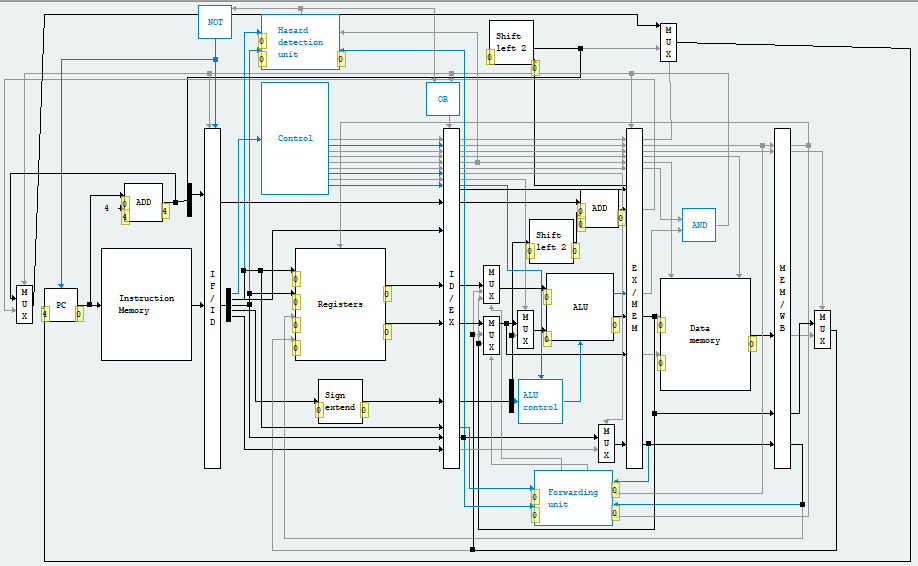
\includegraphics[scale=0.6, center]{J-en-pipeline.png}
    \captionof{figure}{Modificación del data path para el jump}
\end{minipage}

\subsubsection{Instrucción jr en el uniciclo}
Para lograr el jump register se conecto un cable que salia desde ReadData1 de RegBank hacia un multiplexor en la entrada 1 y en la entrada 0 se encuentra la entrada original al PC. Del multiplexor se conecto al Pc.

\begin{minipage}{\linewidth}
   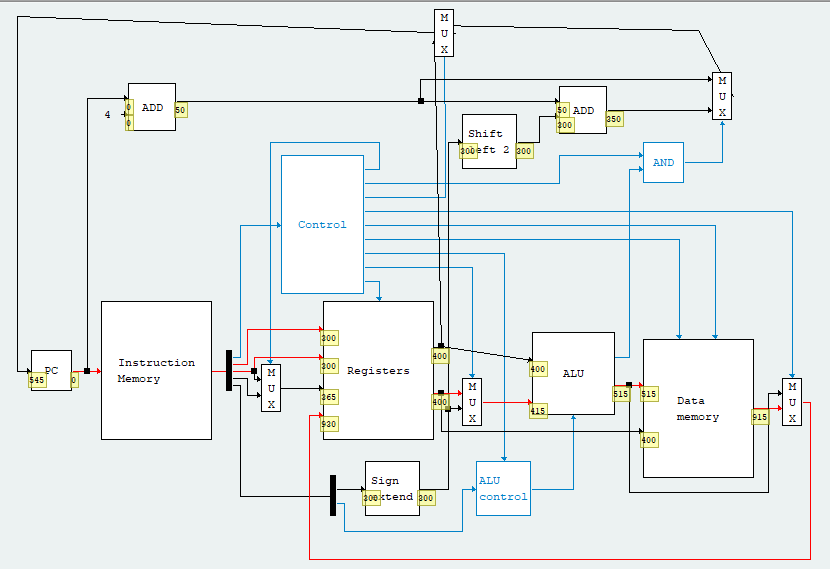
\includegraphics[scale=0.6, center]{jr-unicycle.png}
    \captionof{figure}{Modificación del data path para el jr}
\end{minipage}

\subsubsection{Instrucción jr en el pipeline}
Muy similar al anterior. El registro se saca de ReadData1 del RegBank antes de que se entre al pipeline ID/EX.

\begin{minipage}{\linewidth}
   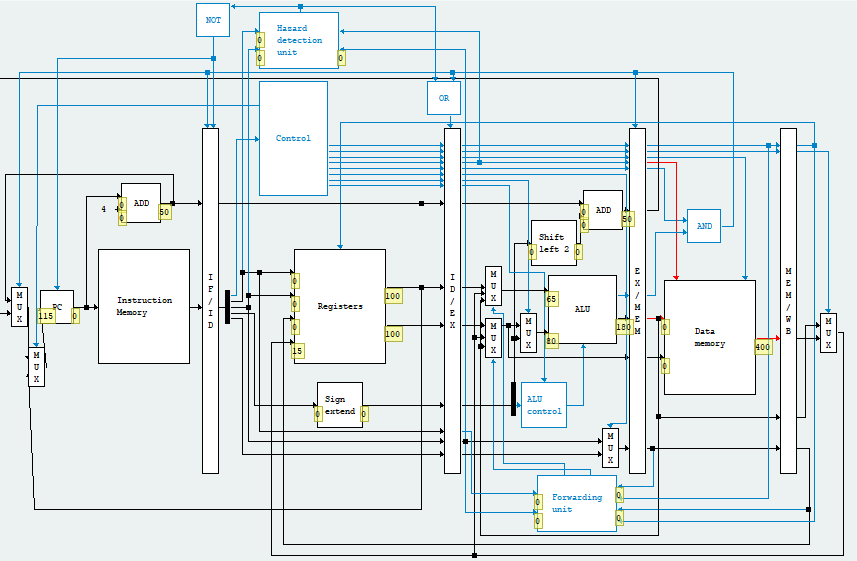
\includegraphics[scale=0.6, center]{jr-pipeline.png}
    \captionof{figure}{Modificación del data path para el jr}
\end{minipage}

\subsubsection{Instrucción jarl en el uniciclo y Instrucción jarl en el pipeline}
Para estos dos no se realizo ninguna modificacion sobre el data path ya que fueron implementados como psudointruciones.

\subsection{Implementacion de las instruciones}
\subsubsection{Instrucción j en el pipeline}
Para la instrucción j se agrego al set de instrucciones la siguiente linea 
\begin{verbatim}
"j":    {"type": "J", "args": ["target"], "fields": {"op": 2, "target": "#1"},
"desc": "PC = target"}
\end{verbatim}
\\
\\ Y se agrego en control lo siguiente:\\ \\"2": {"Jump": 1} \\ \\
En la ejecución del jump en el pipeline genera un hazard que no se pudo corregir. Esto sucede ya que el pipeline mientras se ejecuta una instrucción, ya se empieza a trabajar las siguientes.\\ 
Los ejemplos utilizados para testear fueron: \\ \\
\begin{verbatim}
    j Target
addi $t1, $zero, 5
addi $t2, $zero, 5
addi $t3, $zero, 5
addi $t3, $zero, 5


 Target: 
 	addi $t0, $zero, 5
 	
 	
 	

addi $t0, $zero, 5
j Target
nop
nop
nop
nop
addi $t1, $zero, 5
Target:
	addi $t5, $zero, 5
\end{verbatim}

\subsubsection{Instrucción jr en el uniciclo}
Para esta instruccion se agrego la siguiente linea en el set de intrcciones:\\ \\
"jr": {"type": "R", "args": ["reg"], "fields": {"op": 3, "rs": "#1", "rt": "0", "rd": "0", "shamt": 0, "func": 8}, "desc": "The jr instruction loads the PC register with a value stored in a register."} \\ \\

Y en el control lo siguiente: \\ \\
"3": {"Jump": 1},

La instrucción jarl tiene un campo 0p igual a 3.

El ejemplo para testeo fue: \\ \\
\begin{verbatim}
addi $t0, $zero, 16
jr $t0
addi $t1, $zero, 8
addi $t5, $zero, 8
addi $t4, $zero, 8
\end{verbatim}

\subsubsection{Instrucción jr en el pipeline}
Se agrego lo mismo que en la sección anterior ya que lo que tienen que hacer es lo mismo. Pero en el pipeline se produjo un hazzard a diferencia del Unicycle, dado que a que a medida que esta ejecutando la instrucción ya esta trabajando en otra.

\subsubsection{Instrucción jarl en el uniciclo y Instrucción jarl en el pipeline}
Para estas instrucciones lo que se agrego fue: \\ \\
"jalr": {"args": ["reg", "reg"], "to": ["addi #1, $0, $ra", "jr #2"]},
"jalr": {"args": ["reg"], "to": ["addi 31, $0, $ra", "jr #1"]}
\\ \\ En la sección de pseudo del archivo .set.

El ejemplo para el testeo fue: \\ \\

\begin{verbatim}
addi $t0, $zero, 24
jr $t0
nop
nop
addi $t1, $zero, 8
addi $t5, $zero, 8
addi $t4, $zero, 8
\end{verbatim}

\subsection{Conclusiones}

Este trabajo cumplió el propósito de entender las distintas implementaciones del Data Path al igual que los inconvenientes que cada uno puede tener. Como los jumps y branches que generan hazzards en el pipeline.

\newpage
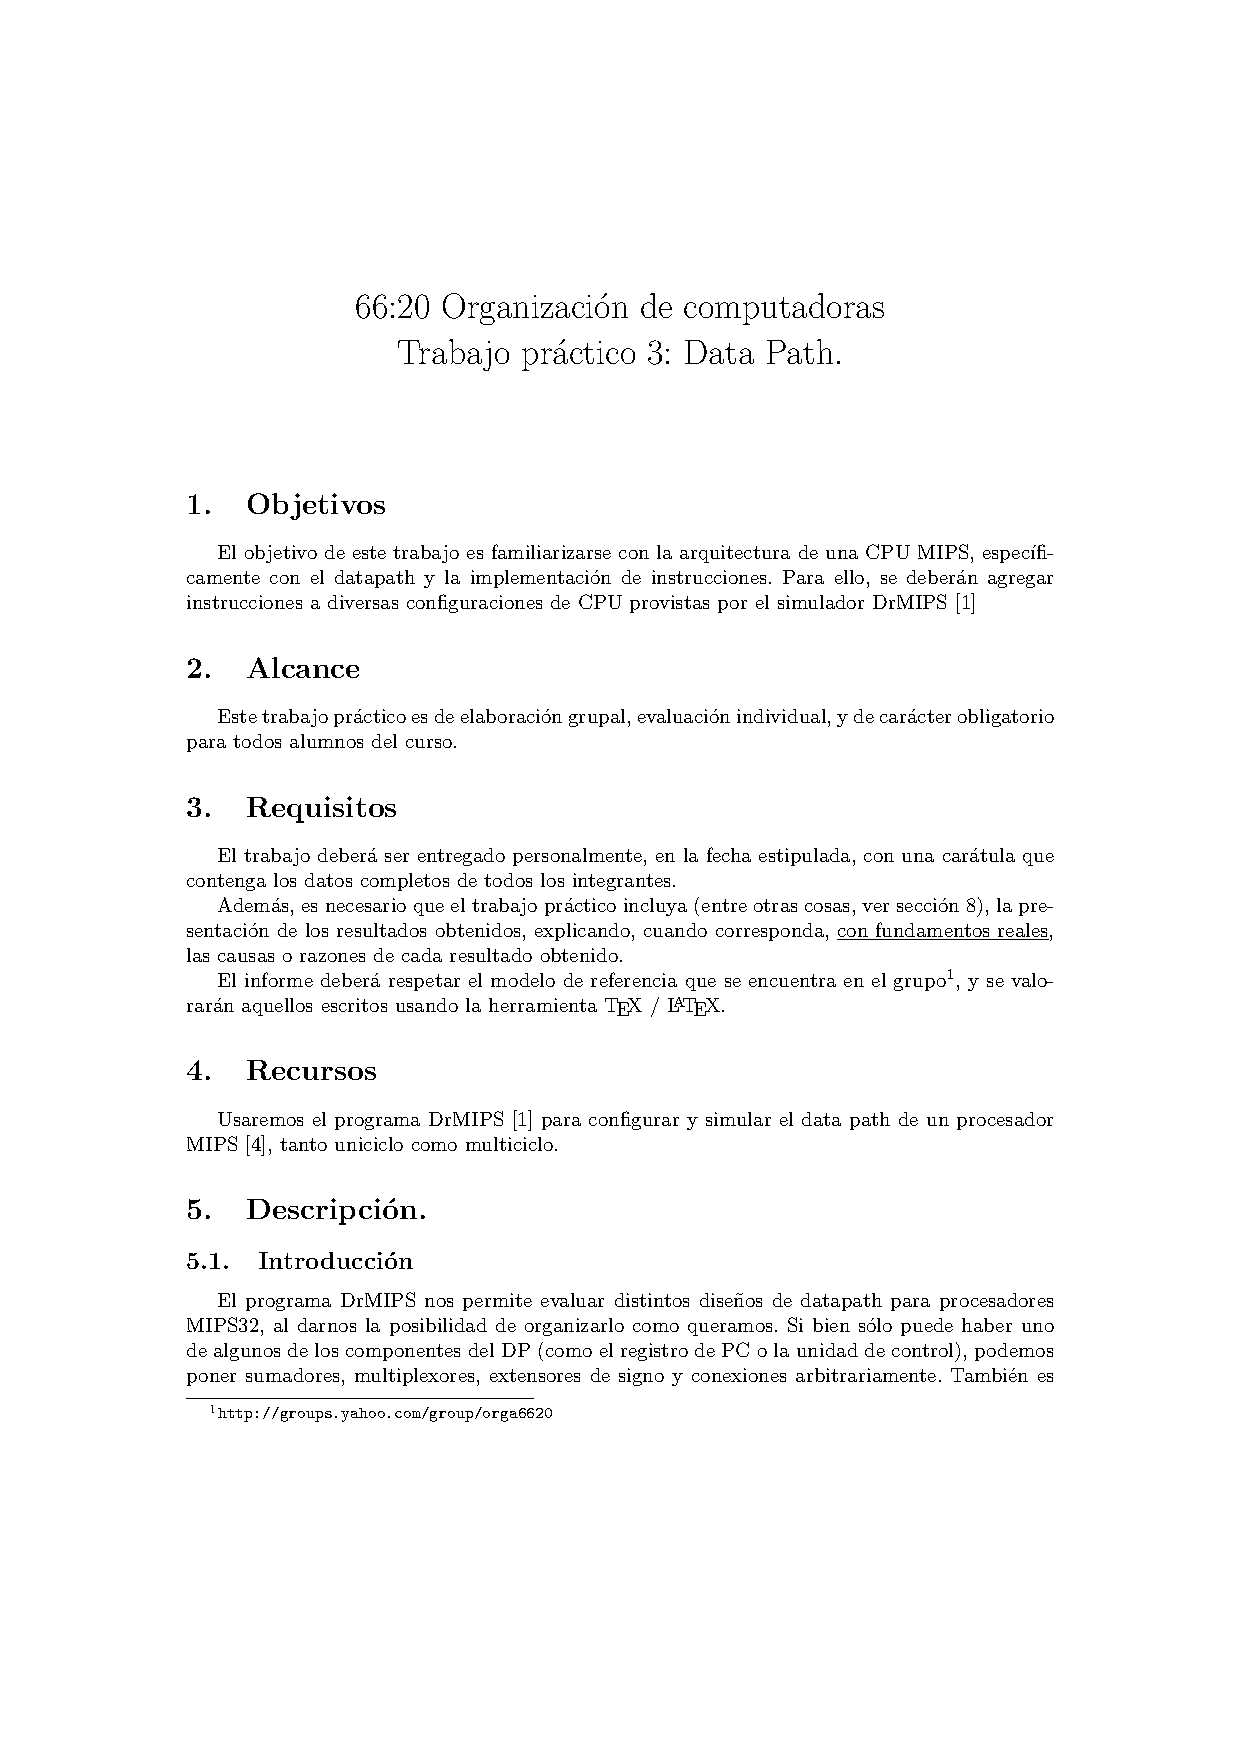
\includepdf[pages=-]{Tp3-q1-2018.pdf}

\end{document}
